% !TeX spellcheck = pl_PL
\documentclass[11pt,a4paper]{article}
\usepackage[utf8]{inputenc}
\usepackage{amsmath}
\usepackage{float}
\usepackage{amsfonts}
\usepackage{mathtools,amssymb,amsthm}
\usepackage{graphicx}
\usepackage{polski}
\mathtoolsset{showonlyrefs,mathic}
\author{Kamil Zawistowski, Michał Cerazy}


\begin{document}
\title{Pakiety statystyczne \\ Sprawozdanie 3}
\author{Michał Cerazy, Kamil Zawistowski \\ 229969, 229924}
\maketitle
\newpage
\tableofcontents
\newpage
\section{Cel}
Celem prowadzonych badań jest odszukanie występowania zależności między statystykami, w koszykówce, przy użyciu modeli regresji. 

\section{Zbiór danych}
Przedmiotem badań są statystyki poszczególnych zawodników występujących na parkietach NBA w sezonie 2014/2015. Podczas tego sezonu w lidze wystąpiło 490 zawodników( każda drużyna może zatrudniać jednocześnie 15 graczy), co przekłada się na taką samą długość próbki. Polecenie wymaga co najmniej 500 pomiarów, jednak w związku z atrakcyjnością omawianych danych, zdecydowaliśmy się na ich użycie. Dane pochodzą ze strony $kaggle.com$. 
\subsection{Opis zmiennych}
Zmienne kategoryczne wyróżnione są poprzez nawiasy zawierające wartości, które zmienna może przyjąć. W sprawozdaniu zostały użyte następujące zmienne:
\begin{itemize}
	\item ,,Name'' -- imię oraz nazwisko,
	\item ,,Age'' -- wiek,
	\item ,,Birth Place'' -- miejsce urodzenia (US, NONUS),
	\item ,,Height''-- wzrost,
	\item ,,Pos'' -- pozycja, na której gra dany zawodnik (PG, SG, C, PF, SF),
	\item ,,Team'' -- ostatni zespół, w którym grał zawodnik,
	\item ,,Weight'' -- waga zawodnika,	
	\item ,,BMI'' -- wskaźnik Body Mass Index, 
	\item ,,Games Played'' - ilość rozegranych meczy w sezonie,	
	\item ,,MIN'' -- ilość minut spędzonych na boisku w sezonie,
	\item ,,PTS'' -- ilość punktów zdobytych w sezonie,
	\item ,,FGM'' -- ilość trafionych rzutów z gry w sezonie,
	\item ,,FGA'' -- ilość rzutów z gry w sezonie,
	\item ,,FGp'' -- procentowa skuteczność rzutów z gry w sezonie,
	\item ,,ThreePM'' -- ilość trafionych rzutów za 3 punkty w sezonie,
	\item ,,ThreePA'' -- ilość rzutów za 3 punkty w sezonie,
	\item ,,ThreePp'' -- procentowa skuteczność rzutów za trzy punkty w sezonie,
	\item ,,FTM'' -- ilość trafionych rzutów osobistych w sezonie,
	\item ,,FTA'' -- ilość rzutów osobistych w sezonie,
	\item ,,FTp'' -- procentowa skuteczność rzutów osobistych w sezonie,
	\item ,,OREB'' -- ilość zbiórek ofensywnych w sezonie,	
	\item ,,DREB'' -- ilość zbiórek defensywnych w sezonie,	
	\item ,,REB'' -- ilość zbiórek w sezonie,
	\item ,,AST'' -- ilość asyst w sezonie,
	\item ,,STL'' -- ilość przechwytów w sezonie,
	\item ,,BLK'' -- ilość bloków w sezonie,
	\item ,,TOV'' -- ilość strat w sezonie,
	\item ,,PF'' -- ilość fauli osobistych w sezonie,
	\item ,,EFF'' -- wydajność zawodnika,
	\item ,,AST/TOV'' -- stosunek ilości asyst do ilości strat,
	\item ,,STL/TOV'' -- stosunek ilości przechwytów do ilości strat.
\end{itemize}
	Dodatkowo, na potrzeby modeli wprowadziliśmy dodatkowe kolumny takie jak:
\begin{itemize}	
	\item ,,PPG'' -- średnia ilość punktów zdobywanych na mecz,
	\item ,,MPG'' -- średnia ilość minut rozegranych na mecz,
	\item ,,FTAPG'' -- średnia ilość rzutów osobistych na mecz,
	\item ,,FGAPG'' -- średnia ilość rzutów z pola na mecz,
	\item ,,ThreeAPG'' -- średnia ilość rzutów za 3 punkty na mecz.
\end{itemize}
%\subsection{Wybór zmiennych zależnych i niezależnych}
%	Jako zmienną zależną będziemy rozważać średnią ilość punktów zdobywanych na mecz. Do zmiennych niezależnych należą !!!! UZUPEŁNIĆ ZMIENNE NIEZALEŻNE !!!!. Decydujemy się na taki wybór, gdyż chcemy poznać wpływ poszczególnych statystyk na liczbę zdobywanych punktów. (?) Odnalezienie odpowiedniego modelu będzie podstawą do wyznaczania zawodników pretendujących do bycia najlepiej punktującymi w kolejnych sezonach. (?)
	
\section{Dopasowanie modelu}
Jako zmienną zależną będziemy rozważać średnią ilość punktów zdobywanych na mecz. Zasugerowane przez nas modele będą się różnić doborem zmiennych niezależnych, jednakże w każdym z nich używać będziemy średniej ilości rozegranych minut na mecz, gdyż jest niezbędna informacja do analizy modelu. Dodatkowo, w naszych modelach będziemy korzystać z cech fizycznych zawodników, statystyk rzutowych, pochodzenia i pozycji, dlatego usuniemy dane dotyczące asyst, bloków, zbiórek, przechwytów, strat i drużyn, w których skończyli sezon.

\subsection{Model I: umiejętności rzutowe zawodników}
Przy pierwszym ze sprawdzanych przez nas modeli skupimy się na zdolnościach rzutowych, a więc zmiennymi objaśniającymi będą średnia ilość rzutów z pola, skuteczność z pola, średnia ilość rzutów za 3 punkty, skuteczność rzutów za 3 punkty, średnia ilość rzutów osobistych, skuteczność rzutów osobistych oraz średnia ilość minut przegranych w meczu. W tabeli \ref{offense} przedstawione zostały wartości współczynników oraz pozostałe statystyki dla omawianego modelu. 
\begin{table}[H]
	\begin{tabular}{| c | c | c | c | c |}
		\hline
		Zmienna & Estymacja & Błąd standardowy & T-wartość & Pr$(<|t|)$\\ \hline
		FGAPG & 0.961931 & 0.025304 & 38.015 & $<$2e-16\\ \hline
		FGp & 0.012008 & 0.003441 & 3.490 & 0.000528\\ \hline
		ThreeAPG & 0.130223 & 0.032714 & 3.981 & 7.93e-05\\ \hline 
		ThreePp & 0.001808 & 0.002931 & 0.617 & 0.537764\\ \hline
		FTAPG & 0.842080 & 0.044256 & 19.027 & $<$2e-16\\ \hline
		FTp  & -0.007247 & 0.002059 & -3.519 & 0.000474\\ \hline
	\end{tabular}
	\caption{Model rzutowy - współczynniki modelu}
	\label{offense}
\end{table}
\begin{figure}[t]
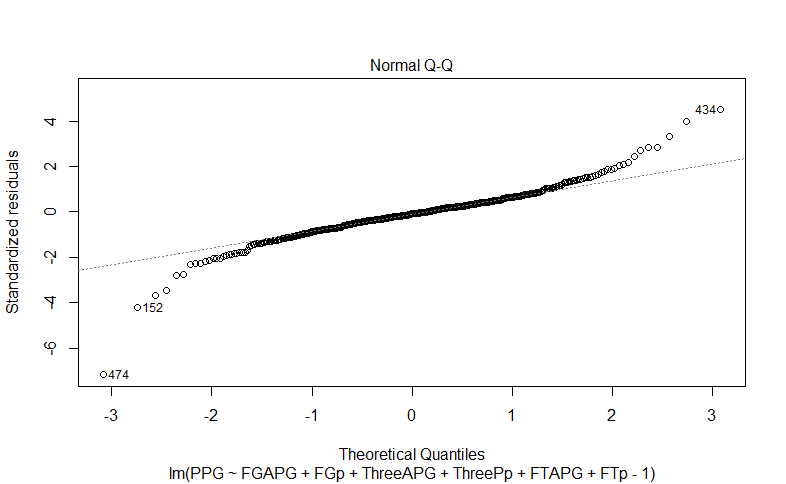
\includegraphics[width=\textwidth]{offense_2}
\caption{QQplot dla modelu rzutowego}
\label{qqplot_offense}
\centering
\end{figure}
Jak można zauważyć, wszystkie parametry poza skutecznością rzutów za 3 punkty są istotne( co może dziwić przy obecnych realiach gry w koszykówkę, gdzie coraz większą wagę przykłada się do szybkich rzutów trzypunktowych). P-value dla testu F wynosi $p-value: < 2.2e-16$, a więc nasz model jest lepszy niż pewna stała. Jak się okazało, w przypadku tego modelu założenia nie są spełnione: test Shapiro-Wilka i spojrzenie na Rysunek \ref{qqplot_offense} odrzuciły hipotezę o normalności residuów, a testy badające stałą średnią i wariancję( polegające na wielokrotnym losowaniu próbki 50 elementów i przeprowadzaniu t.testu i var.testu) wykazały, że średnia jest różna od zera oraz wariancja nie jest stała na poziomie istotności $\alpha=0.05$. Wyniki zawarte zostały w Tabeli \ref{zalozenia_offense}.
\begin{table}[H]
	\begin{tabular}{| c | c | c | c |}
		\hline
		W & p-value & ConstMeanMC & ConstVarMC\\ \hline
		0.92953 & 2.028e-14 & 0.1019 & 0.2892 \\ \hline
	\end{tabular}
	\caption{Model rzutowy - testy założeń}
	\label{zalozenia_offense}
\end{table}
\begin{figure}[t]
	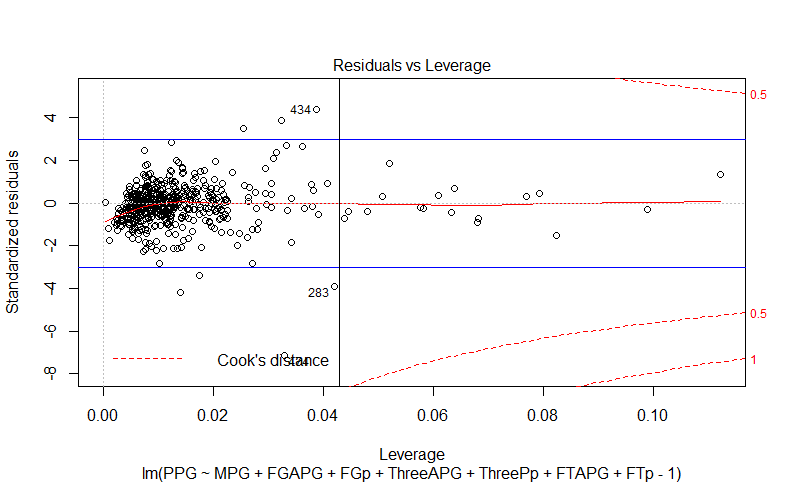
\includegraphics[width=\textwidth]{offense_4}
	\caption{Wykres residuów i dźwigni dla modelu rzutowego}
	\label{leverage_offense}
	\centering
\end{figure}
Na Rysunku \ref{leverage_offense} niebieskimi liniami zaznaczono próg dla wartości odstających, czarną natomiast dla tych o wysokiej dźwigni. Niestety, po ich usunięciu model nadal nie spełniał założeń i pojawiły się kolejne problematyczne obserwacje( próbowaliśmy eliminować je do skutku, jednak nawet to nie przyniosło oczekiwanych rezultatów).
 %pomimo wielokrotnego usuwania tych obserwacji 

\subsection{Model II: pozycje zawodników}
Podczas tworzenia tego modelu staraliśmy się określić, czy pozycja zawodnika wpływa na ilość zdobywanych przez niego punktów, dlatego jako zmienne objaśniające przyjęliśmy pozycję danego gracza, średnią ilość czasu spędzanego na boisku oraz jego wiek.

\begin{figure}[t]
	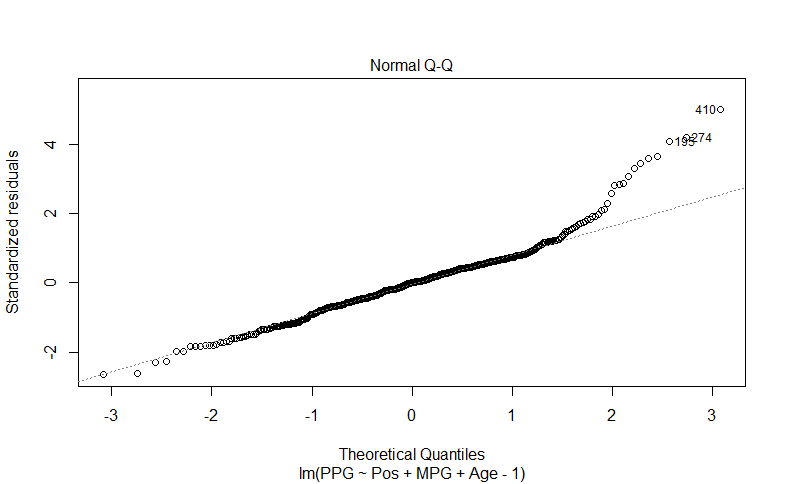
\includegraphics[width=\textwidth]{position_2}
	\caption{QQplot dla modelu uwzględniającego pozycje}
	\label{qqplot_position}
	\centering
\end{figure}
\begin{figure}[t]
	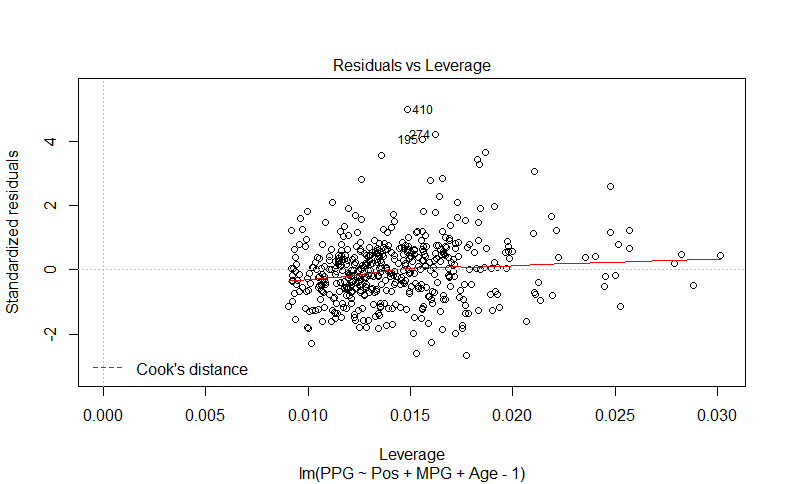
\includegraphics[width=\textwidth]{position_4}
	\caption{Wykres residuów i dźwigni dla modelu uwzględniającego pozycje}
	\label{leverage_position}
	\centering
\end{figure}

\subsection{Model III: pochodzenie zawodników}
Przy ostatnim z badanych modeli chcieliśmy zbadać, czy zawodnicy ze Stanów Zjednoczonych, stanowiący większość ligi, są lepszymi punktującymi niż obcokrajowcy.
Jako zmienne objaśniające przyjęliśmy średnią ilość minut na mecz oraz pochodzenie zawodnika.
\begin{figure}[t]
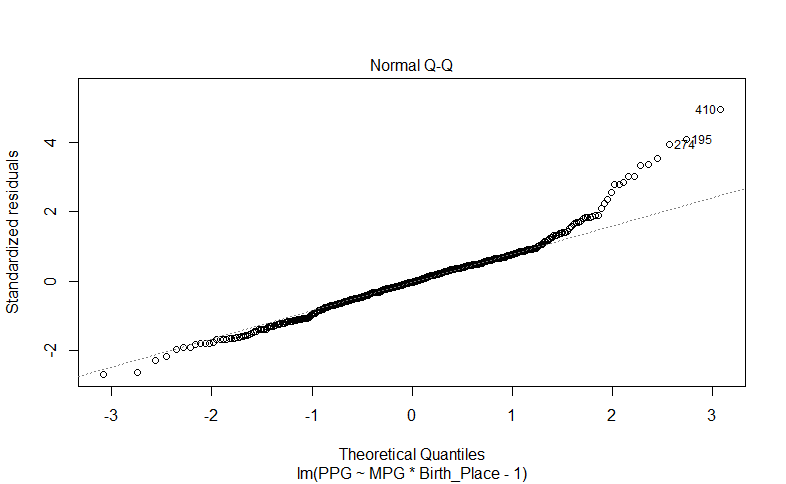
\includegraphics[width=\textwidth]{origin_2}
\caption{QQplot dla modelu uwzględniającego pochodzenie}
\label{qqplot_origin}
\centering
\end{figure}
\begin{figure}[t]
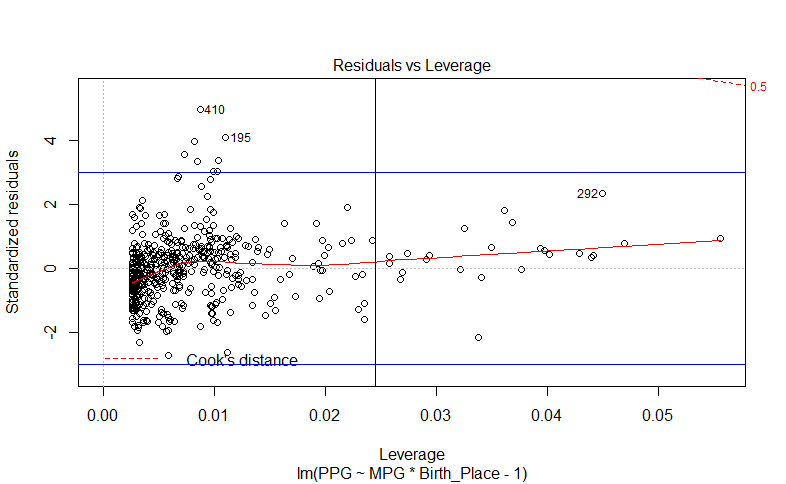
\includegraphics[width=\textwidth]{origin_4}
\caption{Wykres residuów i dźwigni dla modelu uwzględniającego pochodzenie}
\label{leverage_origin}
\centering
\end{figure}

\subsection{Porównanie modeli}
Znając współczynniki dobranych modeli wyznaczyliśmy:
\begin{itemize}
	\item współczynnik determinacji, oznaczany jako $R^2$.
	\item skorygowany współczynnik determinacji, oznaczany jako $aR^2$,
	\item kryterium Akaikego, oznaczane jako $AIC$,
	\item logarytm wskaźnika wiarygodności, oznaczany jako $LogLik$.
\end{itemize}

\begin{table}[H]
	\begin{center}
		\begin{tabular}{| c | c | c | c | c |}
			\hline
			Model & $R^2$ & $aR^2$ & AIC & LogLik \\ \hline
			I & 0.99317 & 0.993 & 1204.576 & -594.288\\ \hline
			II & 0.9374 & 0.9365 & 2283.041 & -1133.52\\ \hline 
			III & 0.9375 & 0.937 & 2281.154 & -1135.577\\ \hline  
		\end{tabular}
		\caption{Porównanie modeli}
		\label{porownanie_modeli}
	\end{center}
\end{table}
Niestety, żaden z dopasowanych modeli nie jest modelem poprawnym, gdyż ich residua nie mają rozkładu normalnego. Sprawdzenia tej hipotezy dokonaliśmy przy użyciu testu Shapiro-Wilka (długość naszej próbki nie przekracza 5000). Statystyka W jest większa od liczby 0.947 (wartość zaczerpnięta z tablic), co implikuje odrzucenie hipotezy zerowej o normalności residuów. W tabeli \ref{porownanie_modeli} widać, że model I cechuje się najlepszym dopasowaniem do danych według wszystkich przedstawionych kryteriów, tak więc możemy założyć, że statystyki rzutowe najlepiej opisują zdobycze punktowe zawodników.

\section{Inne testowane modele}
\subsection{Model uwzględniający cechy motoryczne zawodników}
Podjęliśmy trzy próby dobrania najlepszego modelu, który uzależniony jest od predyspozycji fizycznych zawodników. Oczywiście, model musi być rozszerzony o ilość rozegranych minut na mecz, gdyż jest niezbędna informacja do analizy modelu.

\subsubsection{Model WWW}
Pierwszy z dopasowywanych modeli uwzględnia wzrost, wiek oraz wagę zawodników. Zmienne istotne dla dobranego model to minuty na mecz (jak zakładaliśmy wyżej, jest to najważniejszy czynnik) oraz waga. W tabeli \ref{model_www} przedstawione zostały wartości współczynników oraz pozostałe statystyki dla omawianego modelu. 

\begin{table}[H]
	\begin{tabular}{| c | c | c | c | c |}
		\hline
		Zmienna & Estymacja & Błąd standardowy & T-wartość & Pr$(<|t|)$\\ \hline
		Minuty na mecz & 0.54219 & 0.01242 & 43.638 & $<$2e-16\\ \hline
		Wzrost & -0.03394 & 0.02154 & -1.576 & 0.1156\\ \hline
		Wiek & -0.01660 & 0.02667 & -0.622 & 0.5340\\ \hline 
		Waga & 0.02721 & 0.01462 & 1.861 & 0.0634\\ \hline
		Stała & 1.63120 & 3.35589 & 0.486 & 0.6271 \\ \hline
	\end{tabular}
	\caption{Model WWW - współczynniki modelu}
	\label{model_www}
\end{table}

\subsubsection{Model WW}
Drugi z dopasowywanych modeli uwzględnia wiek oraz wagę zawodników. Odjęcie wzrostu ma na celu sprawdzenie jak zachowa się model po odjęciu jednej zmiennej nie będącej zmienną istotną. W tabeli \ref{model_ww} przedstawione zostały współczynniki modelu WW. Jak można zauważyć zmienne istotne dla modelu nie są już takie same, do minut na mecz dołączyła wartość stała. Ponadto waga zawodnika przestała należeć do istotnych zmiennych.

\begin{table}[H]
	\begin{tabular}{| c | c | c | c | c |}
		\hline
		Zmienna & Estymacja & Błąd standardowy & T-wartość & Pr$(<|t|)$\\ \hline
		Minuty na mecz & 0.54356 & 0.01241 & 43.78 & $<$2e-16\\ \hline
		Wiek & -0.01304 & 0.02661 & -0.490 & 0.62428 \\ \hline 
		Waga & 0.00852 & 0.00857 & 0.994 & 0.32059\\ \hline
		Stała & -3.35012 & 1.13018 & -2.964 & 0.00318\\ \hline
	\end{tabular}
	\caption{Model WW - współczynniki modelu}
	\label{model_ww}
\end{table}

\subsubsection{Model WB}
Trzeci z dopasowywanych modeli uwzględnia wiek oraz wskaźnik BMI. Omawiany wskaźnik jest popularną statystyką mówiącą o stanie zdrowia fizycznego i wyliczana jest na podstawie poniższego wzoru:
\begin{equation}
BMI = \frac{waga}{wzrost^2}.
\end{equation}
W związku z tym niejawnie do modelu włączamy wagę i wzrost zawodników ligi. Wyniki tego zabiegu przedstawione są w tabeli \ref{model_wb}. Podobnie jak w modelu WW istotne zmienne to liczba minut na boisku oraz stała. 
\begin{table}[H]
	\begin{tabular}{| c | c | c | c | c |}
		\hline
		Zmienna & Estymacja & Błąd standardowy & T-wartość & Pr$(<|t|)$\\ \hline
		Minuty na mecz & 0.54259 & 0.01238 & 43.838 & $<$2e-16\\ \hline
		Wiek & -0.01608 & 0.02667 & -0.603 & 0.54676\\ \hline 
		BMI & 0.09639 & 0.05878 & 1.640 & 0.10166\\ \hline  
		Stała & -4.84181 & 1.60703 & -3.013 & 0.00272\\ \hline	
	\end{tabular}
	\caption{Model WB - współczynniki modelu}
	\label{model_wb}
\end{table}
\subsection{Porównanie modeli}
Znając współczynniki dobranych modeli wyznaczyliśmy:
\begin{itemize}
	\item skorygowany współczynnik determinacji, oznaczany jako $R^2$,
	\item kryterium Akaikego, oznaczane jako $AIC$,
	\item logarytm wskaźnika wiarygodności, oznaczany jako $LogLik$,
	\item wartość w z testu Shapiro-Wilka, oznaczana jako $W$.
\end{itemize}

\begin{table}[H]
	\begin{center}
		\begin{tabular}{| c | c | c | c | c |}
			\hline
			Model & $R^2$ & AIC & LogLik & W\\ \hline
			WWW & 0.7977 & 2282.972 & -1135.486 & 0.95495\\ \hline
			WW & 0.7971 & 2283.475 & -1136.737 & 0.95403\\ \hline 
			WB & 0.7978 & 2281.766 & -1135.883 & 0.95493\\ \hline  
		\end{tabular}
		\caption{Porównanie modeli}
		\label{porownanie_modeli_w}
	\end{center}
\end{table}
Każdy z dopasowanych modeli jest ,,poprawnym modelem'', gdyż ich residua mają rozkład normalny. Sprawdzenia tej hipotezy dokonaliśmy przy użyciu testu Shapiro-Wilka (długość naszej próbki nie przekracza 5000). Wartość W jest mniejsza od liczby 0.947 (wartość zaczerpnięta z tablic), co oznacza, że nie ma podstaw by odrzucić hipotezę o normalności residuów. W tabeli \ref{porownanie_modeli_w} widać, że model WB cechuje się najlepszym dopasowaniem do danych według współczynnika $R^2$. Kryterium informacyjne Akaikego również przemawia za wybraniem trzeciego modelu jako najlepiej opisującego badany zbiór wartości. Jedyną statystyką przemawiającą za innym modelem niż WB jest logarytm wskaźnik wiarygodności, który wskazuje, że to pierwszy model jest najlepszy. Na podstawie zaprezentowanych wyników należy wybrać model uwzględniający wiek oraz BMI zawodników.


\section{Podsumowanie}
Model opisujący zdolności rzutowe okazał się być istotnie najlepszym spośród wszystkich testowanych przez nas.  
\end{document}